\section{utentiInteressati(CriteriDiRicercaUtenti request)}

Il metodo \colorbox{lightgray}{utentiInteressati}, appartenente alla classe \colorbox{lightgray}{RicercaAnnunciEffettuatiService}, ha la responsabilità di individuare tutti gli utenti potenzialmente interessati in base alle ricerche che essi hanno precedentemente effettuato.
Questo metodo viene invocato quando il sistema deve inviare una notifica e necessita di filtrare i destinatari realmente pertinenti. Il parametro di ingresso, \colorbox{lightgray}{CriteriDiRicercaUtenti}, contiene i campi relativi alle caratteristiche di un immobile. Se i criteri passati al metodo corrispondono a quelli di una ricerca salvata da un utente nel sistema, tale utente viene incluso nella lista dei destinatari risultanti.
\newline
Per la progettazione dei test unitari è stata adottata una \textbf{strategia di tipo black-box}, analogamente a quanto fatto per il metodo \colorbox{lightgray} {addDipendente}. Tuttavia, la motivazione alla base di questa scelta è differente: mentre nel test di \colorbox{lightgray}{addDipendente} l’obiettivo è verificare che il dipendente aggiunto possieda i valori corretti in funzione della richiesta di input, nel caso di \colorbox{lightgray}{utentiInteressati} l’attenzione è rivolta al comportamento del metodo rispetto ai criteri di ricerca forniti.
In particolare, si verifica che i valori non validi (ad esempio campi vuoti o non significativi) presenti nel parametro \colorbox{lightgray}{CriteriDiRicercaUtenti} vengano opportunamente impostati a \colorbox{lightgray}{null}, in modo da escluderli dal processo di matching con le ricerche salvate. Questo controllo è fondamentale per garantire che il sistema notifichi esclusivamente gli utenti realmente interessati.

Di seguito si riportano le tabelle che documentano tale suddivisione:

\begin{table}[H]
	\centering
	\begin{tabular}{|c|p{4cm}|p{6cm}|c|} 
		\hline
		\textbf{ID Classe} & \textbf{Descrizione} & \textbf{Valore esempio} & \textbf{Validità} \\
		\hline
		A1 & L'insieme delle stringe che corrispondo a una località italiana
		& request.areaDiInteresse==Napoli & Valido \\
		\hline
		A2 & L'insieme delle stringhe null/lunghezza zero
		& request.areaDiInteresse==null & Valido \\
		\hline
		A3 & L'insieme delle stringhe che non corrispondono a una località italiana
		& request.areaDiInteresse==città inesistente & Valido \\
		\hline
	\end{tabular}
	\caption{Parametro request.areaDiInteresse}
	\label{tab:placeholder}
\end{table}

\begin{table}[H]
	\centering
	\begin{tabular}{|c|p{6cm}|p{6.2cm}|c|} 
		\hline
		\textbf{ID Classe} & \textbf{Descrizione} & \textbf{Valore esempio} & \textbf{Validità} \\
		\hline
		C1 & Un valore dell'enumerazione (AFFITTO,VENDITA)
		& request.tipoDiContrattoDiInteresse == AFFITTO; & Valido \\
		\hline
		C2 & valore null
		& request.tipoDiContrattoDiInteresse == null & Valido \\
		\hline
	\end{tabular}
	\caption{Parametro request.tipoDiContrattoDiInteresse}
	\label{tab:placeholder}
\end{table}

\begin{table}[H]
	\centering
	\begin{tabular}{|c|p{6cm}|p{6.2cm}|c|} 
		\hline
		\textbf{ID Classe} & \textbf{Descrizione} & \textbf{Valore esempio} & \textbf{Validità} \\
		\hline
		I1 & Un valore dell'enumerazione
		& request.tipoDiImmobileDiInteresse == APPARTAMENTO; & Valido \\
		\hline
		I2 & valore null
		& request.tipoDiContrattoDiInteresse == null & Valido \\
		\hline
	\end{tabular}
	\caption{Parametro request.tipoDiImmobileDiInteresse}
	\label{tab:placeholder}
\end{table}

\begin{table}[H]
	\centering
	\begin{tabular}{|c|p{4cm}|p{5.5cm}|c|} 
		\hline
		\textbf{ID Classe} & \textbf{Descrizione} & \textbf{Valore esempio} & \textbf{Validità} \\
		\hline
		BMI1 & Qualsiasi numero positivo
		& request.budgetMin==100 & Valido \\
		\hline
		BMI2 & qualsiasi numero negativo
		& request.budgetMin==-100 & Valido \\
		\hline
		BMI3 & valore null
		& request.budgetMin==null & Valido \\
		\hline
	\end{tabular}
	\caption{Parametro request.budgetMin}
	\label{tab:placeholder}
\end{table}

\begin{table}[H]
	\centering
	\begin{tabular}{|c|p{4cm}|p{5.5cm}|c|} 
		\hline
		\textbf{ID Classe} & \textbf{Descrizione} & \textbf{Valore esempio} & \textbf{Validità} \\
		\hline
		BMA1 & Qualsiasi numero positivo
		& request.budgetMan==600 & Valido \\
		\hline
		BMA2 & qualsiasi numero negativo
		& request.budgetMax==-600 & Valido \\
		\hline
		BMA3 & valore null
		& request.budgetMin==null & Valido \\
		\hline
	\end{tabular}
	\caption{Parametro request.budgetMax}
	\label{tab:placeholder}
\end{table}

\begin{table}[H]
	\centering
	\begin{tabular}{|c|p{4cm}|p{5.5cm}|c|} 
		\hline
		\textbf{ID Classe} & \textbf{Descrizione} & \textbf{Valore esempio} & \textbf{Validità} \\
		\hline
		IG1 & Qualsiasi intero positivo & request.intervalloGiorni==10 & Valida \\
		\hline
		II2 & intero negativo & request.intervalloGiorni==-1 & Valido \\
		\hline
		II3 & Valore null & request.intervalloGiorni==null & Valido \\
		\hline
	\end{tabular}
	\caption{Parametro request.intervalloGiorniStoricoRicerche}
	\label{tab:placeholder}
\end{table}

\vspace{1cm}

% Definizione dei colori
\definecolor{bgcolor}{RGB}{245,245,245}    % Sfondo chiaro
\definecolor{keywordcolor}{RGB}{0,0,180}  % Blu per le parole chiave
\definecolor{commentcolor}{RGB}{0,128,0}  % Verde per i commenti
\definecolor{stringcolor}{RGB}{163,21,21} % Rosso per le stringhe


% Configurazione listings
\lstset{
	language=Java,                % Linguaggio di esempio
	backgroundcolor=\color{bgcolor}, % Colore di sfondo
	basicstyle=\ttfamily\small,     % Font e dimensione
	keywordstyle=\color{keywordcolor}\bfseries,
	commentstyle=\color{commentcolor}\itshape,
	stringstyle=\color{stringcolor},
	numbers=left,                   % Numeri a sinistra
	numberstyle=\tiny\color{gray},  % Stile dei numeri
	stepnumber=1,                   % Numeri in ogni riga
	numbersep=5pt,                  % Distanza dai numeri
	frame=single,                   % Cornice intorno al codice
	rulecolor=\color{gray},         % Colore della cornice
	tabsize=4,                       % Tab = 4 spazi
	showstringspaces=false,
	breaklines=true,                  % A capo automatico se troppo lungo
	literate=
		{à}{{\`a}}1
		{è}{{\`e}}1
		{é}{{\'e}}1
		{ì}{{\`i}}1
		{ò}{{\`o}}1
		{ù}{{\`u}}1
}

Prima di ogni test vengono eseguiti i settaggi di deafult della request in modo che venga modificato solo il campo di interesse i ogni test.
Mentre dopo eseguito ogni test viene verificato che alla repository, che interroga il db ed esegue il processo di corrispondenza, vengono passati i parametri che sono impostati nella request. Di seguito mostriamo il codice di tale settaggio.

\begin{lstlisting}
@BeforeEach 
void setup() {
	ricercaAnnunciEffettuataService = new RicercaAnnunciEffettuataService(mockRicercaAnnunciEffettuataRepository,MockUserRepository,new HashSet<String>());
	request = CriteriDiRicercaUtenti.builder()
	.intervalloGiorniStoricoRicerca(10)
	.tipoDiContrattoDiInteresse(TipoContratto.AFFITTO)
	.tipologiaDiImmobileDiInteresse(TipologiaImmobile.APPARTAMENTO)
	.budgetMin(BigDecimal.valueOf(100))
	.budgetMax(BigDecimal.valueOf(600))
	.areaDiInteresse("Napoli")
	.build();
}


@AfterEach 
void verifyRepositorySave() {
	verify(mockRicercaAnnunciEffettuataRepository).trovaUtentiPerCriteri(
	eq(request.getBudgetMin()),
	eq(request.getBudgetMax()),
	eq(request.getAreaDiInteresse()),
	eq(request.getTipoDiContrattoDiInteresse()),
	eq(request.getTipologiaDiImmobileDiInteresse()),
	any(LocalDateTime.class)  // qualsiasi valore va bene
	);
	
	
}
\end{lstlisting}

La suddivisione in classi di equivalenza dei parametri di questo metodo non presenta classi non valide, poiché, come spiegato, i campi con valori non validi vengono impostati a un valore specifico, come ad esempio \colorbox{lightgray}{null}.
La strategia utilizzata per la combinazione dei test consiste nel verificare tutte le classi valide con parametri validi e, successivamente, nell’eseguire un test per ciascun caso in cui un solo campo assume un valore non valido mentre tutti gli altri rimangono validi.


\begin{lstlisting}
	 /**
	* test con area di interesse Italia non deve modificare nulla tranne l'area di interesse che deve settarla a null
	*/
	@Test
	void areaDiInteresseItaliaShouldSetNullAreaDiInteresse() {
		request.setAreaDiInteresse("Italia");
		ricercaAnnunciEffettuataService.utentiInteressati(request);
		assertTrue(request.getAreaDiInteresse()==null);
	}
\end{lstlisting}

\begin{lstlisting}
	/**
	* test che controlla che se il budget max è minore del budget min, li scambia
	*/
	@Test
	void budgetMaxLessThanBudgetMinShouldSwapThem() {
		request.setBudgetMin(BigDecimal.valueOf(600));
		request.setBudgetMax(BigDecimal.valueOf(100));
		ricercaAnnunciEffettuataService.utentiInteressati(request);
		assertTrue(request.getBudgetMin().equals(BigDecimal.valueOf(100)));
		assertTrue(request.getBudgetMax().equals(BigDecimal.valueOf(600)));
	}
\end{lstlisting}

\begin{lstlisting}
	/**
	* Test che controlla che se la città non esiste, imposta a null il campo area di interesse della request
	*/
	@Test
	void invalidCityShouldSetNullAreaDiInteresse() {
		request.setAreaDiInteresse("Città Inesistente");
		ricercaAnnunciEffettuataService.utentiInteressati(request);
		assertTrue(request.getAreaDiInteresse()==null);
	}
\end{lstlisting}

\begin{lstlisting}
	/**
	* test che controlla che se budget min è negativo, lo imposta a null
	*/
	@Test
	void negativeBudgetMinShouldSetNullBudgetMin() {
		request.setBudgetMin(BigDecimal.valueOf(-100));
		ricercaAnnunciEffettuataService.utentiInteressati(request);
		
		assertTrue(request.getBudgetMin()==null);
	}
\end{lstlisting}

\begin{lstlisting}
	/**
	* test che controlla che se budget max è negativo, lo imposta a null
	*/
	@Test
	void negativeBudgetMaxShouldSetNullBudgetMax() {
		request.setBudgetMax(BigDecimal.valueOf(-100));
		ricercaAnnunciEffettuataService.utentiInteressati(request);
		assertTrue(request.getBudgetMax()==null);
	}
\end{lstlisting}

\begin{lstlisting}
	/**
	* test che controlla se l' intervallo di giorni è negativo, lo imposta setta a 7
	*/
	@Test
	void deltaDaysLessThanZeroShouldSet7() {
		request.setIntervalloGiorniStoricoRicerca(0);
		ricercaAnnunciEffettuataService.utentiInteressati(request);
		assertTrue(request.getIntervalloGiorniStoricoRicerca()==7);
		
	}
\end{lstlisting}


\begin{figure}[H]
	\centering
	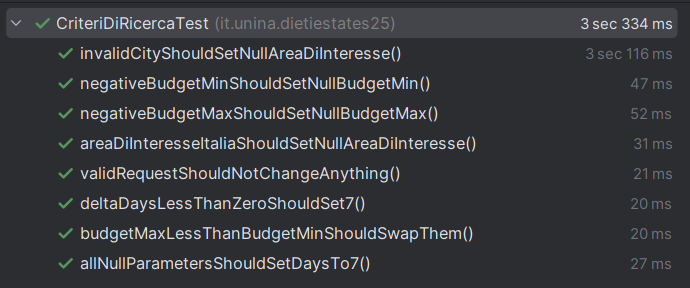
\includegraphics[width=0.7\linewidth]{Immagini/unit test/esitiTestUtentiInteressati.png}
	\caption[Esito test 2]{Screen che riporta l'esito positivo dei test}
\end{figure}
